%\documentclass[12pt, preprint]{aastex}
\documentclass[twocolumn,times]{aastex62}
%\documentclass[preprint,times]{aastex6}

% these lines seem necessary for pdflatex to get the paper size right
\pdfpagewidth 8.5in
\pdfpageheight 11.0in


\usepackage{epsf,color,amsmath}

\usepackage{cancel}

\newcommand{\sfrac}[2]{\mathchoice%
  {\kern0em\raise.5ex\hbox{\the\scriptfont0 #1}\kern-.15em/
    \kern-.15em\lower.25ex\hbox{\the\scriptfont0 #2}}
  {\kern0em\raise.5ex\hbox{\the\scriptfont0 #1}\kern-.15em/
    \kern-.15em\lower.25ex\hbox{\the\scriptfont0 #2}}
  {\kern0em\raise.5ex\hbox{\the\scriptscriptfont0 #1}\kern-.2em/
    \kern-.15em\lower.25ex\hbox{\the\scriptscriptfont0 #2}} {#1\!/#2}}


\newcommand{\castro}{{\sf Castro}}
\newcommand{\maestro}{{\sf Maestro}}

\newcommand{\nablab}{{\mathbf{\nabla}}}
\newcommand{\Ub}{\mathbf{U}}
\newcommand{\gb}{\mathbf{g}}
\newcommand{\omegadot}{\dot{\omega}}
\newcommand{\Sdot}{\dot{S}}
\newcommand{\ddx}[1]{{\frac{{\partial#1}}{\partial x}}}
\newcommand{\ddt}[1]{{\frac{{\partial#1}}{\partial t}}}
\newcommand{\odt}[1]{{\frac{{d#1}}{dt}}}
\newcommand{\divg}[1]{{\nablab \cdot \left (#1\right)}}

\newcommand{\Ic}{\mathcal{I}}
\newcommand{\smax}{{s_\mathrm{max}}}

\usepackage{bm}

\newcommand{\Uc}{{\bm{\mathcal{U}}}}
\newcommand{\Fb}{\mathbf{F}}
\newcommand{\Sc}{\mathbf{S}}

\newcommand{\xv}{{(x)}}
\newcommand{\yv}{{(y)}}
\newcommand{\zv}{{(z)}}

\newcommand{\ex}{{\bf e}_x}
\newcommand{\ey}{{\bf e}_y}
\newcommand{\ez}{{\bf e}_z}

\newcommand{\Ab}{{\bf A}}
\newcommand{\Sq}{{\bf S}_\qb}
\newcommand{\Sqhydro}{{\Sq^{\mathrm{hydro}}}}
\newcommand{\qb}{{\bf q}}

\newcommand{\Shydro}{{{\bf S}^{\mathrm{hydro}}}}
\newcommand{\Rb}{{\bf R}}
\newcommand{\Rq}{{\bf R}}
\newcommand{\Adv}[1]{{\left [\mathcal{A} \left(#1\right)\right]}}
\newcommand{\Advt}[1]{{\left [\mathcal{\tilde{A}} \left(#1\right)\right]}}
\newcommand{\Advs}[1]{{\mathcal{A} \left(#1\right)}}

\setlength{\marginparwidth}{0.75in}
\newcommand{\MarginPar}[1]{\marginpar{\vskip-\baselineskip\raggedright\tiny\sffamily\hrule\smallskip{\color{red}#1}\par\smallskip\hrule}}

\begin{document}
%======================================================================
% Title
%======================================================================
\title{CASTRO: A New Compressible Astrophysical Solver. IV. Performance Portability}

\shorttitle{}
\shortauthors{}

\author{Castro developers / M.~P.~Katz et al.}
\affil{}
\email{}


%======================================================================
% Abstract and Keywords
%======================================================================
\begin{abstract}
We describe a performance portable version of the \castro\ hydrodynamics
code that is able to achieve excellent scaling on both CPU and GPU-based
supercomputers.
\end{abstract}

\keywords{hydrodynamics---methods: numerical}

%======================================================================
% Introduction
%======================================================================
\section{Introduction}\label{Sec:Introduction}

is a compressible (radiation-)hydrodynamics simulation code built on
the AMReX adaptive mesh refinement framework \citep{castro,castro2,castro3}.  It 
includes full self-gravity using multigrid methods with isolated boundaries
\cite{katz:2016}, works with general equations of state \citep{zingalekatz}
and arbitrary nuclear reaction networks.

Existing GPU-enabled astrophysical hydro codes include
\citet{gamer,cholla,fargo3d,pekkila:2017,caplan:2018,racz:2018,liska:2018,goz:2018}

GPU-enabled integration has been explored by \citep{brock:2015}.

Discuss frameworks vs.\ doing it outselves

Discuss OpenMP, OpenACC, and CUDA.

\section{Performance portable compute kernels}

Describe mfiter structure

Describe MPI, MPI+OpenMP w/ tiling, MPI + CUDA

\begin{figure}
\centering
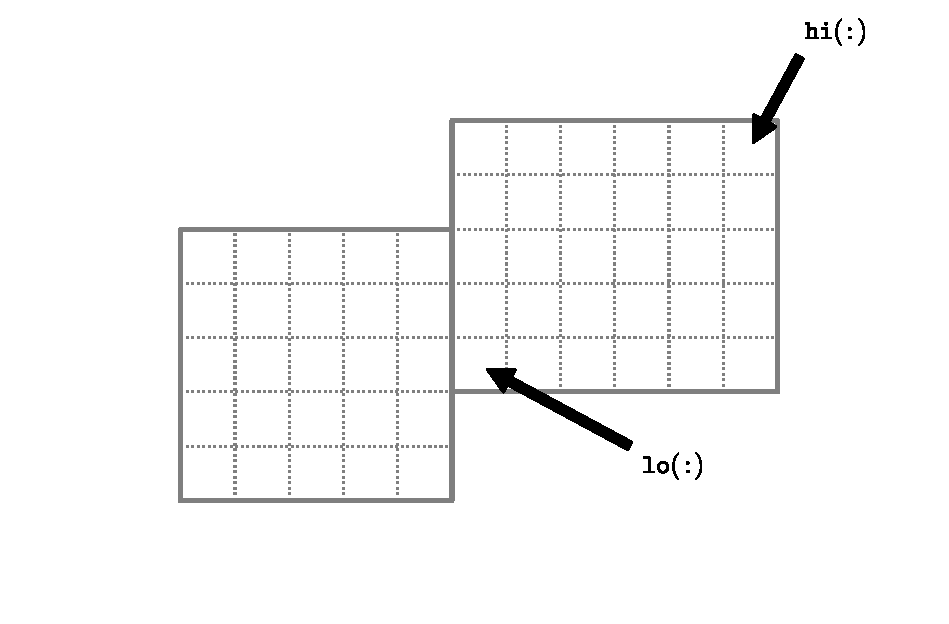
\includegraphics[height=0.25\textheight]{gpu_1} \\
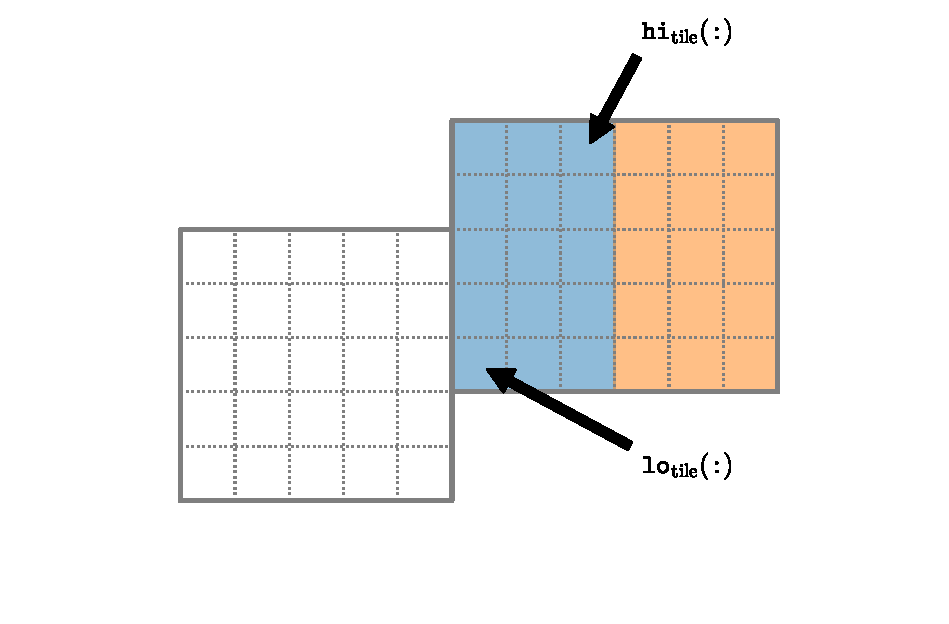
\includegraphics[height=0.25\textheight]{gpu_2} \\
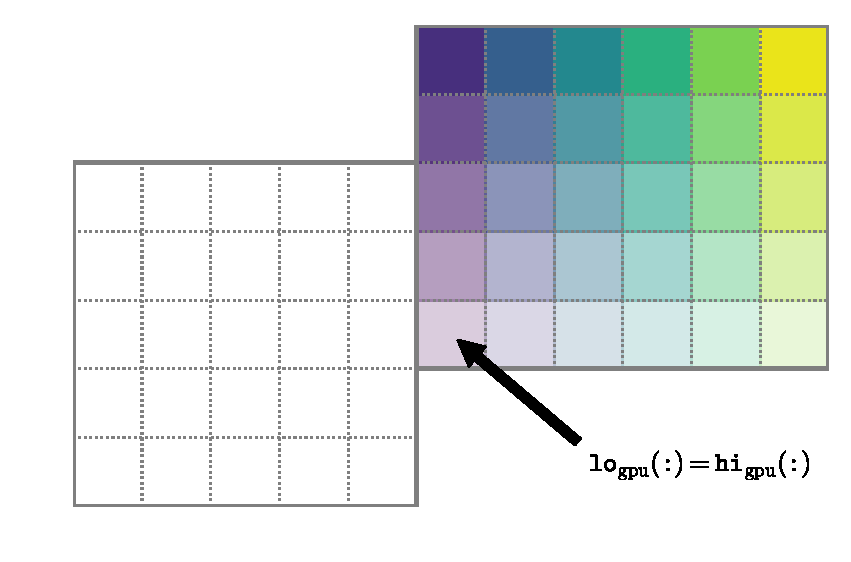
\includegraphics[height=0.25\textheight]{gpu_3}
\caption{\label{fig:loops} caption}
\end{figure}

\subsection{Summary of changes required}

The main hydrodynamics solver in \castro\ is an unsplit corner
transport upwind \citep{ppmunsplit} piecewise parabolic method
\citep{ppm} scheme.  This uses full corner coupling, requiring a 
number of transverse Riemann problem solutions.  

\section{Reaction networks}

\section{Scaling}

Our current focus is on offloading the hydrodynamics and reactions to
GPUs, so we will achieve the best GPU performance for problems without
self-gravity.

\subsection{Pure hydrodynamics}

\subsection{Reaction test}

\subsection{X-ray burst}

This problem uses constant gravity, so all of the physics can be done on the GPUs.


\section{Summary}

Future work: gravity on GPUs (multigrid or multipole), port of \maestro\ following
the same ideas.

\software{MPICH, GCC, Castro, python, matplotlib}

\acknowledgements \castro\ is freely available at
\url{http://github.com/AMReX-Astro/Castro}.  The work at Stony Brook
was supported by DOE/Office of Nuclear Physics grant DE-FG02-87ER40317
and NSF award AST-1211563.  An award of computer time was provided by
the Innovative and Novel Computational Impact on Theory and Experiment
(INCITE) program.  This research used resources of the Oak Ridge
Leadership Computing Facility at the Oak Ridge National Laboratory,
which is supported by the Office of Science of the U.S. Department of
Energy under Contract No. DE-AC05-00OR22725.  We thank NVIDIA Corporation
for the donation of a Titan X Pascal used in this research.





%======================================================================
% References
%======================================================================

\bibliographystyle{apj}
\bibliography{ws}

\end{document}
